\section{Measured Results}
\label{sec:results}

\definecolor{cPass}{HTML}{2E8B7F}
\definecolor{cApp}{HTML}{C0504D}
\definecolor{cAgent}{HTML}{C08A33}
\definecolor{cOther}{HTML}{8C8C8C}
\definecolor{cLine}{HTML}{4F8AA8}

Every figure in this section is reconstructed from the campaign record: five
batch files and 123 trajectory directories, each holding one device execution
step by step. Nothing is reported from memory or from a summary.

\keypoint{Two of the targets belong to third parties who are not party to this
engagement, and are identified here as AUT-1 and AUT-2 rather than by name.
AUT-1 is a production agricultural-commerce marketplace with live users, built
with a cross-platform toolkit that exposes almost no stable accessibility
identifiers. AUT-2 is an institutional form and survey platform. Every count,
verdict and technical claim about them is reproduced unmodified from the
campaign record. The remaining three targets are public applications and are
named.}

\subsection{Autonomy}

Autonomy is the share of executions that end in a statement about the
application rather than a failure of our agent. It is reported first because
every other number depends on it.

\begin{figure}[H]
  \centering
  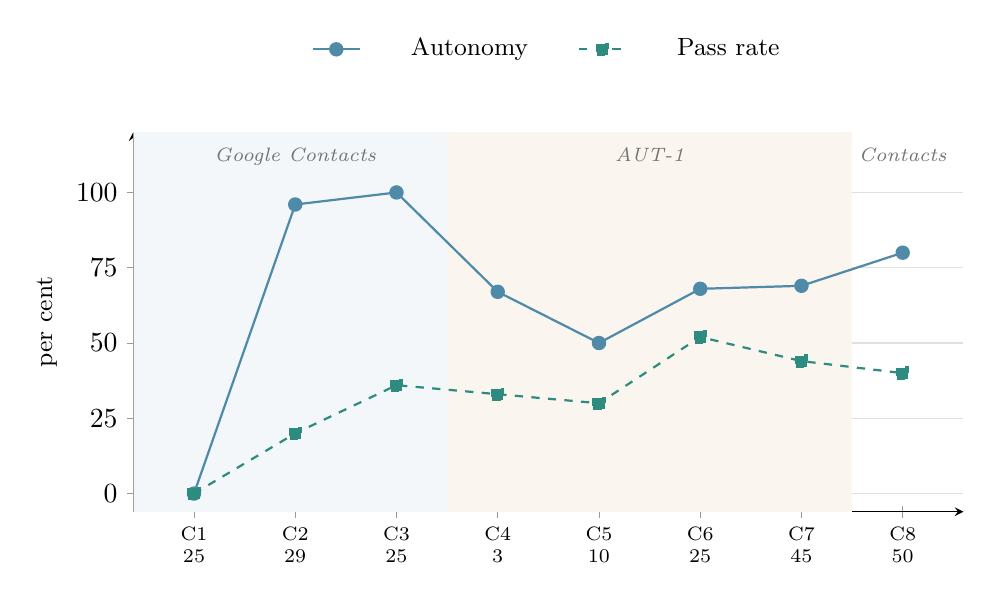
\begin{tikzpicture}
    \begin{axis}[
      width=\textwidth, height=6.4cm,
      ymin=-6, ymax=120, ytick={0,25,50,75,100},
      ylabel={per cent}, ylabel style={font=\small},
      xmin=0.4, xmax=8.6, xtick={1,2,3,4,5,6,7,8},
      xticklabels={{C1\\\scriptsize 25},{C2\\\scriptsize 29},{C3\\\scriptsize 25},%
                   {C4\\\scriptsize 3},{C5\\\scriptsize 10},{C6\\\scriptsize 25},%
                   {C7\\\scriptsize 45},{C8\\\scriptsize 50}},
      xticklabel style={align=center, font=\scriptsize},
      ymajorgrids, grid style={black!12}, axis lines=left, tick style={black!40},
      legend style={at={(0.5,1.16)}, anchor=south, legend columns=2,
                    font=\small, draw=none, fill=none, column sep=1.6em},
    ]
      \fill[cLine!7] (axis cs:0.4,-6) rectangle (axis cs:3.5,120);
      \fill[cAgent!8] (axis cs:3.5,-6) rectangle (axis cs:7.5,120);
      \node[font=\scriptsize\itshape, text=black!55, anchor=north] at (axis cs:2.0,118) {Google Contacts};
      \node[font=\scriptsize\itshape, text=black!55, anchor=north] at (axis cs:5.5,118) {AUT-1};
      \node[font=\scriptsize\itshape, text=black!55, anchor=north] at (axis cs:8.0,118) {Contacts};
      \addplot[cLine, thick, mark=*, mark size=2.2pt]
        coordinates {(1,0) (2,96) (3,100) (4,67) (5,50) (6,68) (7,69) (8,80)};
      \addplot[cPass, thick, dashed, mark=square*, mark size=2.0pt]
        coordinates {(1,0) (2,20) (3,36) (4,33) (5,30) (6,52) (7,44) (8,40)};
      \legend{Autonomy, Pass rate}
    \end{axis}
  \end{tikzpicture}
  \caption[Autonomy across every instrumented campaign]{Autonomy and pass rate
  across all eight instrumented campaigns in the order they were run, with the
  number of tests under each. The target is shaded behind the lines.}
  \label{fig:autonomy}
\end{figure}

The first instrumented campaign, C1, returned a 0\,\% pass rate, which read at
first as a catastrophic quality result. It was not. Eighty-two per cent of device
steps could not be parsed, so almost nothing could be attributed. The
instrumentation worked and revealed that the evidence did not. Four fixes
closed the gap: log reassembly so a step is written once
and completely, containment matching so a screen is recognisable without stable
identifiers, a precondition filter so tests are not issued against states the
application cannot be in, and a device reset so one test cannot contaminate the
next. Two campaigns later, on the same target, the system recorded 100\,\%
autonomy and zero silent fallbacks.

Autonomy then fell when the agent was pointed at AUT-1, reaching 67\,\% and then 50\,\%. We report this rather than
presenting the best result alone, because it is the more useful fact for
anyone planning to deploy the system: a tuned agent does not transfer for free.
Recovery to 68\,\% came from the structural state-identity work, and the two
full campaigns that followed settled at 69\,\% on AUT-1 and 80\,\% on
Contacts.

\keypoint{Across all eight campaigns the pass-rate line moves far less than the
autonomy line. What improved over this period was mostly the agent's ability to
reach a verdict at all, which is the capability that had to come first.}

\subsection{Transfer across targets}

Five targets were exercised across both platforms. None required a code change.

\begin{figure}[H]
  \centering
  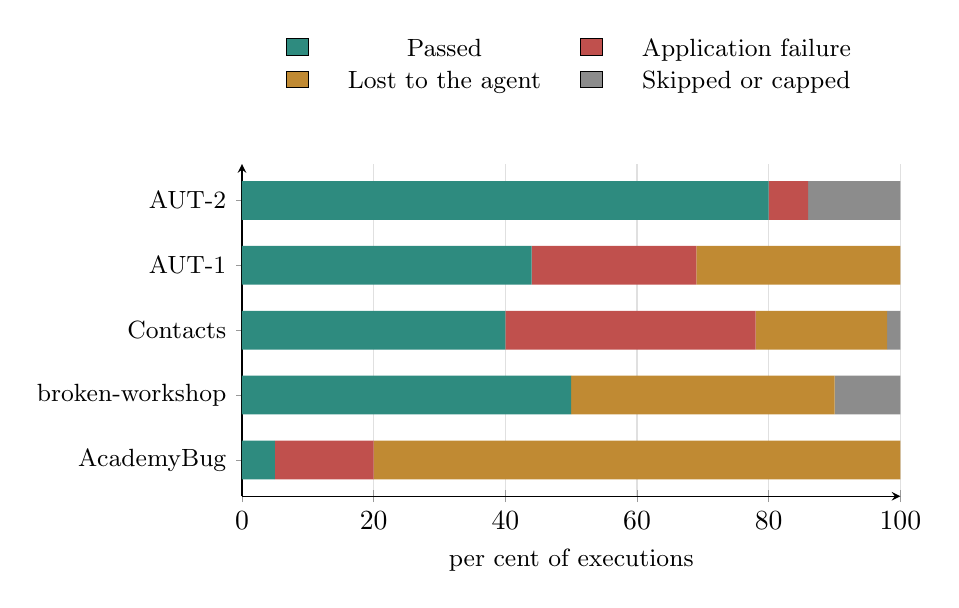
\begin{tikzpicture}
    \begin{axis}[
      width=0.82\textwidth, height=5.8cm,
      xbar stacked, xmin=0, xmax=100,
      xlabel={per cent of executions}, xlabel style={font=\small},
      bar width=14pt,
      symbolic y coords={AcademyBug, broken-workshop, {Contacts}, {AUT-1}, AUT-2},
      ytick=data, yticklabel style={font=\small},
      xmajorgrids, grid style={black!12}, axis lines=left,
      tick style={black!40}, enlarge y limits=0.14,
      legend style={at={(0.5,1.18)}, anchor=south, legend columns=2,
                    font=\small, draw=none, fill=none, column sep=1.2em},
    ]
      \addplot[fill=cPass,  draw=none] coordinates {(80,AUT-2) (44,{AUT-1}) (40,{Contacts}) (50,broken-workshop) (5,AcademyBug)};
      \addplot[fill=cApp,   draw=none] coordinates {(6,AUT-2)  (25,{AUT-1}) (38,{Contacts}) (0,broken-workshop)  (15,AcademyBug)};
      \addplot[fill=cAgent, draw=none] coordinates {(0,AUT-2)  (31,{AUT-1}) (20,{Contacts}) (40,broken-workshop) (80,AcademyBug)};
      \addplot[fill=cOther, draw=none] coordinates {(14,AUT-2) (0,{AUT-1})  (2,{Contacts})  (10,broken-workshop) (0,AcademyBug)};
      \legend{Passed, Application failure, Lost to the agent, Skipped or capped}
    \end{axis}
  \end{tikzpicture}
  \caption[Outcome attribution across five targets]{Outcome attribution as a
  share of executions. The amber band is the one to read first: it is the share
  of runs that say nothing about the application because the agent failed.}
  \label{fig:targets}
\end{figure}

\begin{table}[H]
  \centering\small
  \setlength{\tabcolsep}{4pt}
  \begin{tabularx}{\textwidth}{@{}>{\hsize=0.56\hsize}Y>{\hsize=0.28\hsize}Y>{\hsize=0.24\hsize}Y>{\hsize=0.30\hsize}Y>{\hsize=0.30\hsize}Y>{\hsize=1.32\hsize}Y@{}}
    \toprule
    Target & Platform & Tests & App fail & Agent & Coverage and wall clock \\
    \midrule
    AUT-2 & Web & 64 & 4 & \textbf{0} & 51 passed, 7 skipped, 2 capped \\
    \addlinespace
    AUT-1 & Android & 45 & 11 & 14 & 33/106 requirements, 29 areas, 97 UI states; 7.5\,h \\
    \addlinespace
    Google Contacts 4.86.23 & Android & 50 & 19 & 10 & 55/141 requirements, 35 areas, 60 UI states; 6.2\,h \\
    \addlinespace
    broken-workshop & Web & 10 & 0 & 4 & 170 steps, 1 capped; 51\,min \\
    \addlinespace
    AcademyBug & Web & 20 & 3 & \textbf{16} & no specification ingested; 50\,min \\
    \bottomrule
  \end{tabularx}
\end{table}

\paragraph{AUT-2.} Fifty runs against an institutional form and survey
platform produced 64 judged test cases: 51 passed, 4 product failures, nothing
at all attributed to the agent. A campaign in which the tester never becomes
the explanation for a failure, reproduced on a platform and a domain the tuning
was not done against. The findings were one critical, a notifications control
absent from the workspace header, and three major concerning a sidebar control
that failed to open its view.

\paragraph{Google Contacts.} An application no member of the team had any hand
in, tested against an independently written 141-requirement specification
rather than a vendor document. The agent designed 50 test cases for an
application it had never seen, executed each on a device, and returned 19
application-level failures and 125 findings about the application.

\paragraph{AUT-1.} The production marketplace, and the hardest target,
for structural reasons. Its cross-platform toolkit exposes almost no stable
identifiers and reports one activity per screen. It also carries live users, so
a class of operations was blocked in configuration rather than exercised.
Within those limits it produced 11 application-level failures, 95 findings, and
97 mapped interface states, the most of any target.

\paragraph{The two that went badly.} On broken-workshop, a deliberately faulty
web application, ten tests were run, five completed, and zero defects were
found. Whether the faults lay outside the reachable surface or were simply not
provoked cannot be determined from the record. On AcademyBug, 16 of 20 runs
were lost to the agent. No specification was ingested for that target, so the
coverage line reads zero of zero requirements. The two results together are the
clearest statement we can make about the value of a specification.

\subsection{Effort, and what it buys}

\begin{figure}[H]
  \centering
  \begin{subfigure}{0.48\textwidth}
    \centering
    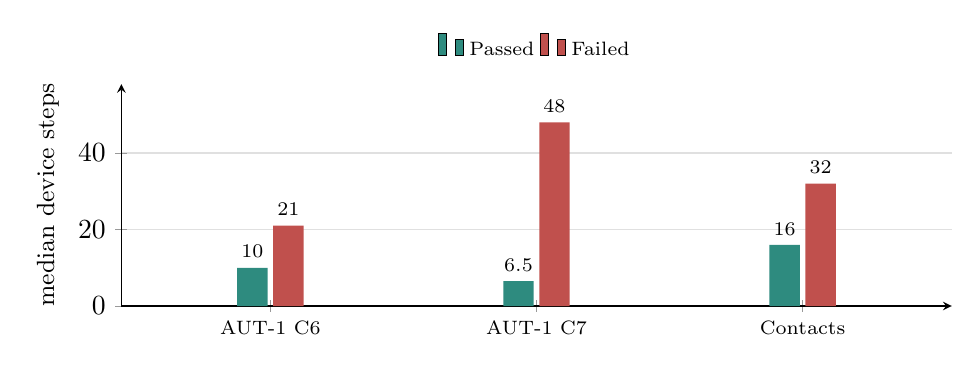
\begin{tikzpicture}
      \begin{axis}[
        width=\textwidth, height=4.4cm,
        ybar, bar width=11pt, ymin=0, ymax=58,
        ylabel={median device steps}, ylabel style={font=\small},
        symbolic x coords={{AUT-1 C6},{AUT-1 C7},{Contacts}}, xtick=data,
        xticklabel style={font=\scriptsize},
        ymajorgrids, grid style={black!12}, axis lines=left,
        tick style={black!40}, enlarge x limits=0.28,
        nodes near coords, nodes near coords style={font=\scriptsize\bfseries},
        legend style={at={(0.5,1.06)}, anchor=south, legend columns=2,
                      font=\scriptsize, draw=none, fill=none},
      ]
        \addplot[fill=cPass, draw=none] coordinates {({AUT-1 C6},10) ({AUT-1 C7},6.5) ({Contacts},16)};
        \addplot[fill=cApp,  draw=none] coordinates {({AUT-1 C6},21) ({AUT-1 C7},48) ({Contacts},32)};
        \legend{Passed, Failed}
      \end{axis}
    \end{tikzpicture}
    \caption{Median steps by verdict.}
    \label{fig:stepsverdict}
  \end{subfigure}\hfill
  \begin{subfigure}{0.48\textwidth}
    \centering
    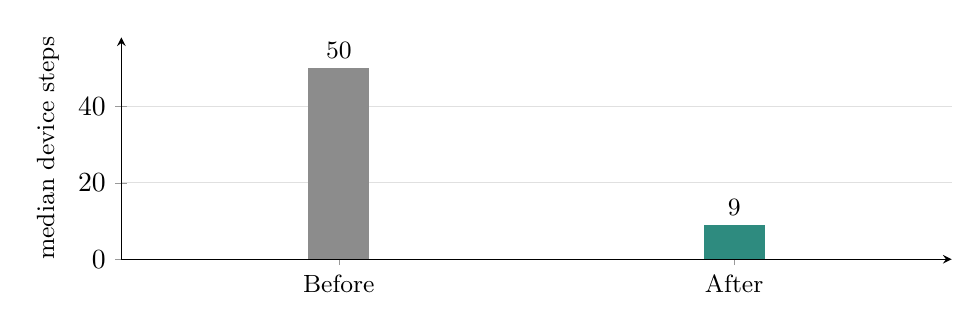
\begin{tikzpicture}
      \begin{axis}[
        width=\textwidth, height=4.4cm,
        ybar, bar width=22pt, ymin=0, ymax=58,
        ylabel={median device steps}, ylabel style={font=\small},
        symbolic x coords={Before, After},
        xtick={Before,After}, bar shift=0pt,
        xticklabel style={font=\small},
        ymajorgrids, grid style={black!12}, axis lines=left,
        tick style={black!40}, enlarge x limits=0.55,
        nodes near coords, nodes near coords style={font=\small\bfseries},
      ]
        \addplot[fill=cOther, draw=none] coordinates {(Before,50)};
        \addplot[fill=cPass, draw=none] coordinates {(After,9)};
      \end{axis}
    \end{tikzpicture}
    \caption{Effect of navigation memory.}
    \label{fig:steps}
  \end{subfigure}
  \caption[Device steps]{Left: a test that is going to pass reaches its
  checkpoint quickly, and a test that is going to fail spends its whole budget.
  On the full AUT-1 campaign the gap is 6.5 steps against 48, with
  an interaction cap of 50, so the median failing test is running to the cap
  rather than reaching a verdict. Right: navigation memory cut the overall
  median from 50 steps to 9.}
  \label{fig:effort}
\end{figure}

Two consequences follow from the left-hand panel. Cost is concentrated in the
runs that produce the least evidence, so raising the step cap raises cost
faster than it raises findings, and the right lever is better navigation rather
than a larger budget. And the shape is diagnostic: a campaign whose failing
tests cluster at the cap has a navigation problem, while one whose failures are
short has an application problem.

\subsection{One campaign, test by test}

\begin{figure}[H]
  \centering
  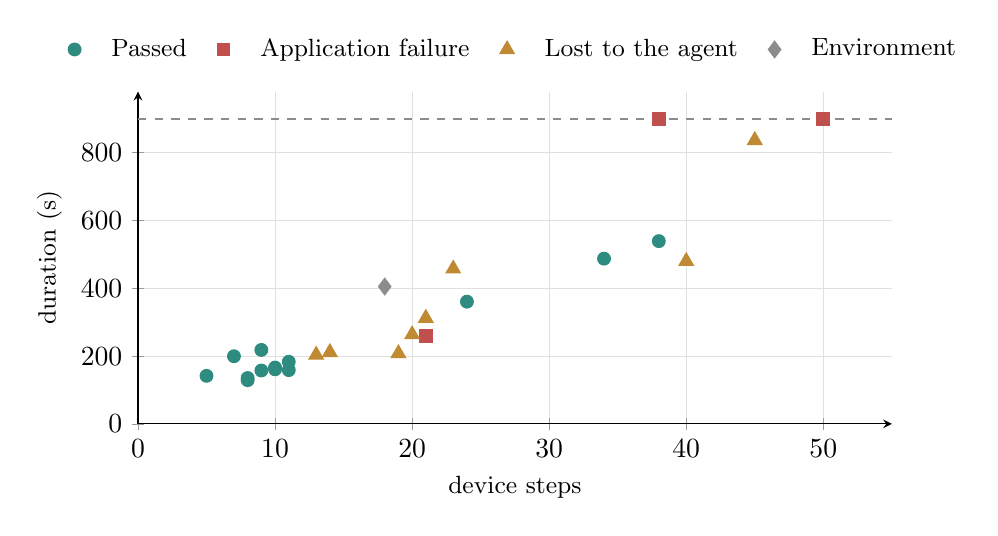
\begin{tikzpicture}
    \begin{axis}[
      width=0.92\textwidth, height=5.8cm,
      xmin=0, xmax=55, ymin=0, ymax=980,
      xlabel={device steps}, ylabel={duration (s)},
      xlabel style={font=\small}, ylabel style={font=\small},
      xmajorgrids, ymajorgrids, grid style={black!12},
      axis lines=left, tick style={black!40},
      legend style={at={(0.5,1.06)}, anchor=south, legend columns=4,
                    font=\small, draw=none, fill=none, column sep=0.9em},
    ]
      \addplot[only marks, mark=*, mark size=2.3pt, color=cPass]
        coordinates {(38,539.2) (8,135.3) (11,183.3) (24,360.6) (10,166.2) (7,199.6)
                     (10,161.0) (8,129.0) (34,487.5) (11,158.7) (9,218.2) (5,141.7) (9,157.5)};
      \addplot[only marks, mark=square*, mark size=2.3pt, color=cApp]
        coordinates {(38,900.2) (21,258.1) (50,900.1)};
      \addplot[only marks, mark=triangle*, mark size=3pt, color=cAgent]
        coordinates {(19,207.8) (40,480.0) (13,203.5) (23,457.6) (14,211.1)
                     (20,263.6) (21,312.0) (45,836.7)};
      \addplot[only marks, mark=diamond*, mark size=3pt, color=cOther]
        coordinates {(18,405.2)};
      \addplot[dashed, black!45, thick, forget plot] coordinates {(0,900) (55,900)};
      \legend{Passed, Application failure, Lost to the agent, Environment}
    \end{axis}
  \end{tikzpicture}
  \caption[Every test in one campaign]{All 25 tests of campaign C6, plotted by
  the steps taken and the time consumed. The dashed line is the
  900-second wall-clock cap. Steps and duration are close to proportional at
  about eleven seconds per step, which is why step count is used as the cost
  proxy throughout this report.}
  \label{fig:scatter}
\end{figure}

Failures occupy the upper right: they consume the most time and the most steps
to produce the least evidence. The dominant failure mode in this campaign was
navigation livelock, eight of the twelve failures, where the agent oscillated
between screens without progressing.

\subsection{Findings and coverage}

Both large Android campaigns produced far more findings than tests, because a
single run yields several observations. Of 163 findings on AUT-1, 95
describe the application; of 198 on Contacts, 125 do. The remainder record the
agent's own difficulties or questions a run raised but could not settle.
Reporting the totals as defect counts would overstate by roughly 40\,\%, and
the separation is enforced rather than left to a reader.

Requirement coverage was 31\,\% on AUT-1 and 39\,\% on Contacts.
Feature-area coverage was substantially higher, 29 and 35 areas respectively.
Coverage is reported at a given spend rather than as a quantity that is ever
complete, because exploratory testing has no natural stopping point.

\subsection{How long a campaign takes}

Unit cost is cheap and wall clock is not. The Contacts campaign took 6.2 hours
for 50 tests and AUT-1 7.5 hours for 45, at medians of 346 and 476
seconds per test. A campaign of this size is most of a working day of device
time, which places it in a nightly run rather than in a pre-commit gate.

The time is dominated by the device rather than by the models. At roughly
eleven seconds of wall clock per device step, only a fraction of which is spent
waiting on inference, the cost of a campaign in elapsed time is emulator time.
Running several emulators in parallel against one planner is the obvious
remedy and is discussed in \Cref{sec:economics}.
